\section{Experiment}\label{sec:experiment}

We carried out our evaluation on a desktop PC, running Windows 7 with Intel Core i5, 2410 Mhz processor, and 4 GB of RAM. 
%We have implemented test selection techniques and mutant generation in Java.
%We generate mutants by changing rules
%in access control policies.
For our test selection approach, we use test selection based on mutation analysis ($Mut$-$Selection$),
test selection based on coverage analysis ($Cov$-$Selection$), and
test selection based on recorded request evaluation ($Req$-$Selection$)
described in Section~\ref{sec:approach}.

For regression, we simulate policy evolution by changing/adding/removing rules in access control policies.
We do not simulate regression in test code in subjects. For evaluation,
our implementation randomly chooses one of regression types, which are RMR, RA,
and CRE, and feeds such change in the rule. We configured that our implementation
to inject 5, 10, 15, 20, and 25 changes in a policy, respectively.
%We conducted our evaluation for 10 times to 
Our evaluation is repeated for 12 times in order to avoid the impact of randomness of changes.

To measure the effectiveness of our three techniques,
we measure how many test cases are reduced for regression testing.
To measure the efficiency of our three techniques, we conducted evaluation as follows. 
We compared elapsed time to analyze test-rule correlation analysis,
change impact analysis, and test selection by each technique.
For the first two techniques, we require test-rule correlation analysis
and change impact analysis, which should be done before actual test selection.
The objective of this evaluation is to investigate how our three test selection techniques impacts performance for subjects.
To measure the effectiveness of our test augmentation technique,
we measure test coverage with selected and new augmented test cases.

%We compare also selected tests by our three techniques to
%compare that all of these techniques return the same tests for regression.



%\textbf{Detection: -- selection detection two Type} evaluated result inconsistency and number of reqs (in case of dependency) or failure trace info
  
%
%
%\begin{figure}[t]
%    \centering
%        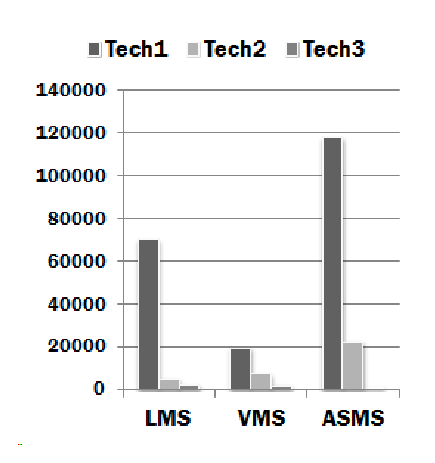
\includegraphics[width=2.0in]{test-rule.eps}
%        \vspace{-5pt}
%    \caption{\label{fig:framework} ACPT overview}
%    \vspace{-10pt}
%%    \vspace{+3pt}
%\end{figure}

%\begin{figure}[t]
%    \centering
%        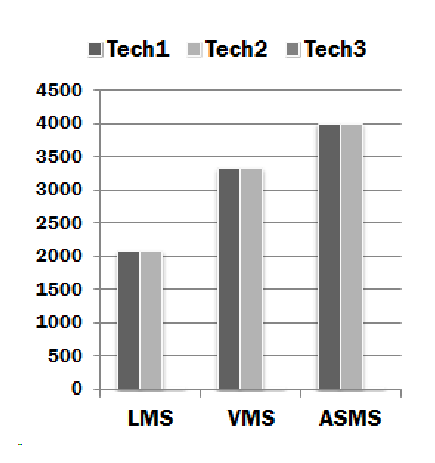
\includegraphics[width=2.0in]{testselection.eps}
%        \vspace{-5pt}
%    \caption{\label{fig:framework} ACPT overview}
%    \vspace{-10pt}
%%    \vspace{+3pt}
%\end{figure}


\begin{table*}[tbp]
  \centering
  	\caption{Subjects used in our evaluation}
  	\vspace{-8pt}    
    \begin{tabular}{|l|r|r|r||r|r|r|}
    \hline
    	\multirow{2}{*}{Subjects} & \multirow{2}{*}{LOC} & \multicolumn{2}{|c||}{ \# Test Methods} & \multicolumn{3}{|c|}{AC Rule Coverage} \\\cline{3-7}
    
          &  & \# Total & \# Security Tests & \# Cov & \# Not-Cov& \% Cov\\\hline\hline
    LMS   & 3749  & 46    & 29    & 42    & 0     & 100 \\\hline
    VMS   & 3734  & 52    & 10    & 13    & 106   & 12 \\\hline
    ASMS  & 7836  & 93    & 91    & 109   & 21    & 83 \\\hline
		\end{tabular}%
  \label{tab:subj}%
%\end{table}%
%
%\begin{table*}[tbp]

\vspace{+10pt}

  \centering
  \caption{Policy statistics used in our subjects}
  	\vspace{-8pt}   
    \begin{tabular}{|l|r|r|r|r||r|r|r|}
 		\hline
 		     \multirow{2}{*}{Subject} & \multicolumn{4}{|c||}{Attributes} & \multicolumn{3}{|c|}{\# AC Rules} \\\cline{2-8}
 		     
     & ~\# Subjects~ & ~\# Actions~ & ~\# Resources~ & ~\# Conditions~ & ~\# Explicit~ & ~\# Implicit~ & ~\# Total~ \\\hline\hline
    LMS   & 6     & 10    & 3     & 4     & 42    & 678   & 720 \\\hline
    VMS   & 7     & 15    & 3     & 3     & 106   & 839   & 945 \\\hline
    ASMS~  & 8     & 11    & 5     & 4     & 129   & 1631  & 1760 \\\hline
 
    \end{tabular}%
  \label{tab:subjectpolicies}%
\end{table*}%



% Table generated by Excel2LaTeX from sheet 'Test Reduction'
%\begin{table*}[tbp]
%  \centering
%  \caption{Add caption}
%    \begin{tabular}{|r|r|r|r|r|r|rrrrrrrrrr}
%    \multicolumn{1}{c}{\multirow{2}[4]{*}{Subjects}} & \multicolumn{3}{c}{Regression - 5} & \multicolumn{3}{c}{Regression - 10} & \multicolumn{3}{c}{Regression - 15} & \multicolumn{3}{c}{Regression - 20} & \multicolumn{3}{c}{Regression - 25} & \\
%    \multicolumn{1}{c}{} & \# Counter & \# Covered & \% Covered & \# Counter & \# Covered & \% Covered & \# Counter & \# Covered & \% Covered & \# Counter & \# Covered & \% Covered & \# Counter & \# Covered & \% Covered \\
%    LMS   & 5.00  & 2.42  & 48.33 & 9.00  & 4.75  & 52.78 & 13.00 & 6.25  & 48.08 & 17.42 & 7.75  & 44.50 & 20.67 & 8.83  & 42.74 \\
%    VMS   & 4.92  & 0.42  & 8.47  & 9.25  & 0.67  & 7.21  & 13.83 & 1.33  & 9.64  & 18.92 & 1.08  & 5.73  & 23.75 & 1.75  & 7.37 \\
%    ASMS  & 5.00  & 1.92  & 38.33 & 9.75  & 4.75  & 48.72 & 14.42 & 7.33  & 50.87 & 18.67 & 9.42  & 50.45 & 23.33 & 12.08 & 51.79 \\
%    \end{tabular}%
%  \label{tab:addlabel}%
%\end{table*}%



\subsection{Subjects}
The subjects include three real-life Java programs each, which
interacts with access control policies \cite{testcase}. We next describe
our three subjects.
\begin{itemize}	
\item Library Management System (LMS) provides web services to manage books in a public library.
\item Virtual Meeting System (VMS) provides web conference services. VMS allows users to organize
online meetings in a distributed platform.
\item Auction Sale Management System (ASMS) allows users to buy or sell items on line. A seller initiates an auction by submitting a description of an item she wants to sell with its expected minimum price. Users then participate in bidding process by
bidding the item. For the bidding on the item, users have enough money in her account before bidding.
\end{itemize}

%Table~\ref{tab:subj} shows information in our subjects.
Our subjects use a Sun PDP \cite{sunxacml} to evaluate requests against a policy.
Sun PDP is popularly used PDP to evaluate requests.
Table~\ref{tab:subj} summarizes the basic statistics of our subjects. The first column shows the subject names.
Columns 2-5 show the lines of code (``LOC''), the numbers of total test cases (``\# Total''), security test cases (``\# Security Tests''),
rules covered with existing test cases (``\# Cov''), rules not-covered with existing test cases (``\# Not-Cov''), and the percentage
of rule coverage (``\% Cov''), respectively. For coverage, we refer rules are explicitly specified rules.
In addition, over all of existing test cases, we distinguish security test cases, which issue
more than one request to the PDP from test cases without interaction of policies.

Table~\ref{tab:subjectpolicies} summarizes the basic statistics of policies in our subjects.
The first column shows the subject names.
Columns 2-5 show the numbers of subjects, actions, resources, conditions, explicitly specified rules, implicit
 rules, and total rules for each policy.
The largest one consists of 129 rules.
For explicitly specified rules, developers first write rules for denying or permitting access
explicitly. Implicit rules refer to rules are evaluated in a given policy, while the developers do not write such rules.
For example, In Figure~\ref{fig:example}, Line 34
specifies a rule. This rule denies all the requests $R_d$ that do not match with its preceding rules while
no rules (i.e., implicit rules) are specified to handle such requests explicitly.


\subsection{Objectives and Measures}
In the evaluation, we intend to answer the following research questions:
\begin{itemize}


	\item RQ1: How many of test cases in a test suite (from an existing test suite) selected by our test selection techniques? This question helps to show that our techniques can reduce a significant number of test cases in an existing test suit.
	We also show how many changed policy behaviors are covered with our selected test cases.
	
%	\item RQ2: Do our protest selections are safe? This question helps to show that our techniques select all tests, which shows only and all test cases to reveal changed behaviors in access control policies.
	
	\item RQ2: What are elapsed time for our techniques to conduct test selection by given subjects? This question helps to compare performance of our techniques by measuring efficiency with regards to elapsed time.
			
	\item RQ3: How higher we can achieve additional policy coverage ratio by our test augmentation technique?  This question helps to show that our technique can generate/augment test suite to cover 100\% of changed policy behaviors. We also compare our approach with random test generation technique to show how effectively our approach augment test suite to cover not-coverted changed policy behaviors.
				
\end{itemize}

%\subsection{Metrics}
%
%We use following 4 metrics in our evaluation.
%\begin{itemize}
%	\item Policy coverage information for changed policy behaviors.
%	\item Number of test cases reused by the test selection technique.
%	\item Elapsed time of test-rule correlation, change impact analysis, and test selection.
%	\item Number of test cases generated by the test augmentation technique. 
%\end{itemize}



\begin{table*}[tbp]
  \centering
  \caption{Coverage results of test cases selected for changed policy behaviors for each policy}
  	\vspace{-8pt}   
    \begin{tabular}{|l|r|r|r||r|r|r||r|r|r||r|r|r||r|r|r|}
%\multirow{2}{*}{Subject} & \multicolumn{3}{c}{Regression - 5} & \multicolumn{3}{c}{Regression - 10} & \multicolumn{3}{c}{Regression - 15} & \multicolumn{3}{c}{Regression - 20} & \multicolumn{3}{c}{Regression - 25} & \\
\hline
     \multirow{2}{*}{Subject} & \multicolumn{3}{|c||}{Regression - 5} & \multicolumn{3}{|c||}{Regression - 10} & \multicolumn{3}{|c||}{Regression - 15} & \multicolumn{3}{|c||}{Regression - 20} & \multicolumn{3}{|c|}{Regression - 25} \\\cline{2-16}
       & \# CT & \# Cov & \% Cov & \# CT & \# Cov & \% Cov & \# CT & \# Cov & \% Cov & \# CT & \# Cov & \% Cov & \# CT & \# Cov & \% Cov \\\hline\hline
    LMS   & 5.0   & 2.4   & 48.3  & 9.0   & 4.8   & 52.8  & 13.0  & 6.3   & 48.1  & 17.4  & 7.8   & 44.5  & 20.7  & 8.8   & 42.7 \\\hline
    VMS   & 4.9   & 0.4   & 8.5   & 9.3   & 0.7   & 7.2   & 13.8  & 1.3   & 9.6   & 18.9  & 1.1   & 5.7   & 23.8  & 1.8   & 7.4 \\\hline
    ASMS  & 5.0   & 1.9   & 38.3  & 9.8   & 4.8   & 48.7  & 14.4  & 7.3   & 50.9  & 18.7  & 9.4   & 50.4  & 23.3  & 12.1  & 51.8 \\\hline\hline
    Average & 4.97  & 1.58  & 31.71 & 9.33  & 3.39  & 36.23 & 13.75 & 4.97  & 36.19 & 18.33 & 6.08  & 33.56 & 22.58 & 7.56  & 33.97 \\\hline

    \end{tabular}%
  \label{tab:cov-results}%
\end{table*}%

%techniques as test selection based on mutation analysis ($Mut-Selection$)
%test selection based on coverage analysis ($Cov-Selection$)
%test selection based on recorded rrequest evaluation ($Req-Selection$)

% Table generated by Excel2LaTeX from sheet 'Performance'
\begin{table*}[tbp]
  \centering
  \caption{Elapsed time for each step of test selection technique, and each policy}
  	\vspace{-8pt}   
    \begin{tabular}{|l|r|r|r||r|r|r||r|r|}

			\hline
       \multirow{2}{*}{Subject}   & \multicolumn{3}{|c||}{Mut-Selection} & \multicolumn{3}{|c||}{Cov-Selection} & \multicolumn{2}{|c|}{Req-Selection} \\\cline{2-9}

%          & Pre-computed & \multicolumn{2}{c}{Post-computed} & Pre-computed & \multicolumn{2}{c}{Post-computed} & Pre-computed & Post-computed \\\cline{2-7}
          & TEST-Rule & CIA & Test Selection & TEST-Rule & CIA& Test Selection & Req Collection & Test Selection \\\hline\hline
%    LMS   & 70496 & 2083.333333 & 4.25  & 5214  & 2083.333 & 4.25  & 2096  & 1.933333 \\\hline
%    VMS   & 19771 & 3333.333333 & 0.766667 & 7506  & 3333.333 & 0.766667 & 1873  & 1.866667 \\\hline
%    ASMS  & 118248 & 4000  & 11.36667 & 22423 & 4000  & 11.36667 & 1064  & 20.7 \\\hline

		LMS   & 70496 & 2083  & 4     & 5214  & 2083  & 4     & 2096  & 2 \\\hline
    VMS   & 19771 & 3333  & 1     & 7506  & 3333  & 1     & 1873  & 2 \\\hline
    ASMS  & 118248 & 4000  & 11    & 22423 & 4000  & 11    & 1064  & 21 \\\hline\hline
    Average & 69505 & 3139  & 5     & 11714 & 3139  & 5     & 1678  & 8 \\\hline

    
    \end{tabular}%
  \label{tab:performance-results}%
\end{table*}%

\begin{figure}[t]
    \centering
        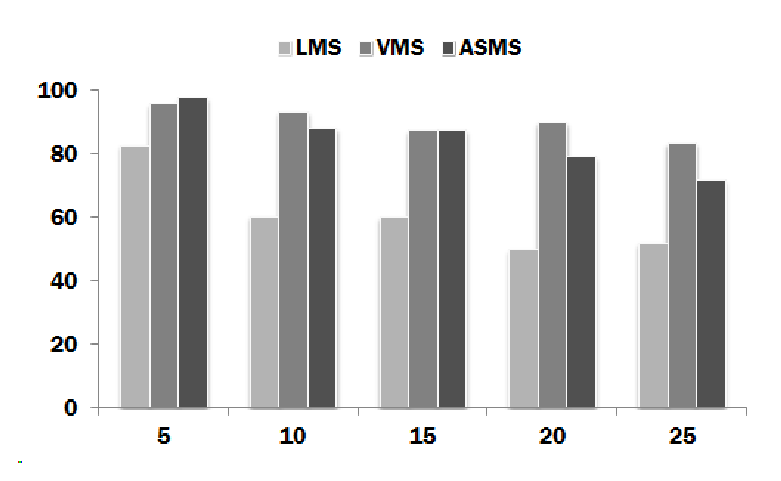
\includegraphics[width=3.0in]{reduction.eps}
        \vspace{-5pt}
    \caption{\label{fig:reduction} Regression test selection results (test reduction) for our subjects and each modified version. Y axis
    denotes the percentage of test reduction. X axis denote the number of policy changes in modified policy of our subjects.}
    \vspace{-10pt}
%    \vspace{+3pt}
\end{figure}

\subsection{Results}
To answer $RQ1$, 
we measure how many test cases are reduced for regression testing.
The goal of this research question is to show the reduction in the number of test cases that
are selected using our techniques. The reduction in the number
of test cases is the same across our three techniques.
Figure~\ref{fig:reduction} shows the results of test reduction for the three subjects.
We observe that 82\%-97\% of test reduction for a modified version with 5 policy changes.
We observe that 51\%-83\% of test reduction for a modified version with 25 policy changes.
Such test reduction may reduce a significant cost in terms of test execution time
for regression testing. We found that all of our test techniques show the same
set of selected test cases to show that all of our techniques can detect every
test case impacted policy changes.

To answer $RQ2$, we measure how many test cases are reduced for regression testing.
The goal of this research question is to compare performance of our three
test selection techniques.
Table~\ref{tab:performance-results} shows the results, which is elapsed time for the three subjects and
each technique.
For $Mut$-$Selection$ and $Cov$-$Selection$, the table shows the elapsed time of
test-rule correlation (``Test-Rule''), change-impact-analysis (``CIA''), and test
selection (``Test Selection''), respectively.
For $Req$-$Selection$, the table shows the elapsed time of
request recording (``Req-Collection''), and test
selection (``Test Selection'').
Note that ``Test-Rule'' and ``Req-Collection'' are preliminary step that could
be done before test selection. 
We observe that $Cov$-$Selection$ (on average 11714 milliseconds) a significant
elapsed time compared to $Mut$-$Selection$ (on average 69505 milliseconds) in terms of test-rule correlation.
Moreover, we observe that a total elapsed time of $Req$-$Selection$ is 43 and 8 times
faster than those of $Mut$-$Selection$  and $Cov$-$Selection$, respectively.


%$Mut$-$Selection$ and $Cov$-$Selection$ show
%elapsed time 69505 (mm) and 11714 (mm) for test-rule correlation.
% $Cov$-$Selection$  


%the reduction in the number of test cases that
%are selected using our techniques.
%
%To measure the efficiency of our three techniques, we conducted evaluation as follows. 
%We compared elapsed time to analyze test-rule correlation analysis,
%change impact analysis, and test selection by each technique.
%For the first two techniques, we require test-rule correlation analysis
%and change impact analysis, which should be done before actual test selection.
%The objective of this evaluation is to investigate how our three test selection techniques impacts performance for subjects.



Table~\ref{tab:cov-results} shows the results for the three subjects.
For each subject, the table shows the number of
changed policy behaviors (``\# CT''), test
cases that were selected (``\# Cov''), and the percentage of test
cases that were selected (``\% Cov'') for each version of its policy.
We denote our modified version of a policy as ``Regression - N'' where
$N$ denotes the number of changes injected into the policy.
``\# CT'' is equal or less than $N$ because our injected changes may not introduce
policy behavior changes at the final modified version of the policy. For example, if one changes
one rule with $CRE$ and again changes the rule with $CRE$. As the results, the rule does not impact
on policy changes.

In Table~\ref{tab:cov-results}, we observe that our selected test cases
cover 31.71-36.23\% of changed policy behaviors. The result show
that about 70\% of changed policy behaviors (i.e., rules impacted by policy changes) are not covered.
We apply our test augmentation technique to add new test cases
to cover such not-covered-rules.

[TBD:Results-test augmentation]

%selects test cases
%
%
%DT , Basic and P rioritization
%detect averagely 25.9%, 62.3%, and 62.3% 


%changes may not lead to.



%The data in the gure illustrate that the reduction in the
%number of selected test cases varies widely both across and
%within the subjects.


%techniques as test selection based on mutation analysis ($Mut$-$Selection$)
%test selection based on coverage analysis ($Cov$-$Selection$)
%test selection based on recorded rrequest evaluation ($Req$-$Selection$)


%Test Suite Reduction. The goal of this study was
%to determine the reduction in the number of test cases that
%could be achieved using our regression-test-selection tech-
%nique. For each subject program P, and each version P',
%we used Retest, shown in Figure 8, to select test cases for
%regression testing.


%
%For each subject, the gure shows the percentage of test
%cases that were selected for each version of that subject.
%The data in the gure illustrate that the reduction in the
%number of selected test cases varies widely both across and
%within the subjects.
%
%Study 2: Safe --------
%
%Whether this result is safe or not. We also compute empirically,
%test dependency and failed together. Okay.
%
%Study 3: Performance ------------ Graph.
%we show that, our testing results is good.
%
%Study 4: augumentation
%
%
%
%	
%[ToDo: explain more]

% Table generated by Excel2LaTeX from sheet 'Sheet1'


%Metrics # of code
%Metrics # of rules in a policy
%Metrics # of system tests
%	seucrity tests
%	selected tests


%In our evaluation, we measure request processing time by evaluating randomly
%generated requests developed by our previous work~\cite{Xengine}.
%In particular, for multiple PDPs, our approach fetches a PEP with a corresponding
%PDP for a given request at run time. Therefore, request processing time includes
%both fetching time and request evaluation time.


%\begin{figure*}[h!]
%  \centering
%  \subfloat[LMS]{\label{fig:gull}\includegraphics[width=0.33\textwidth]{LMS.pdf}}                
%  \subfloat[VMS]{\label{fig:VMS}\includegraphics[width=0.33\textwidth]{VMS.pdf}}
%  \subfloat[ASMS]{\label{fig:ASMS}\includegraphics[width=0.33\textwidth]{ASMS.pdf}}
%  \caption{Request Processing Time for our subjects LMS, VMS and ASMS}
%  \label{fig:processing time}
%\end{figure*}

%\subsection{Performance Improvement Results}\label{subsec:performanceimprovement}
%
%We generated the resulting sub-policies for all the splitting criteria defined in Section~\ref{subsec:SplittingCriteria}.
%For each splitting criteria, we have conducted systems tests to generate requests that trigger all the PEPs in the evaluation. 
%The test generation step leads to the execution of all combination of possible requests described in our previous work \cite{testcase}.  
%The process of tests generation is repeated for ten times in order to avoid the impact of randomness.
%We applied this process to each splitting criterion and calculated evaluation time on average of a system under tests.

\subsection{Threats to Validity}
The threats to external validity primarily include the degree to
which the policies and regression model are representative of true practice.
These threats
could be reduced by further experimentation on a wider type of policy-based software systems and
larger number of policies.
[TBD...]

%In particular, lower-level mutation operators are needed to
%operate on the subject, resource, and action attributes found in various policy elements. Currently the proposed mutation operators
%operate only on higher-level policy elements. Additional mutation
%operators are needed to exploit policy and rule evaluation order as
%well as the numerous functions that may be speci?ed in the condition. The threats to internal validity are instrumentation effects
%that can bias our results such as faults in Sun��s XACML implementation, faults in Margrave��s API and/or its limitations, as well
%as faults in our own policy mutator, policy coverage measurement
%tool, and request generators.

